\RequirePackage[hyphens]{url}
\documentclass{deliverablereport}

\deliverable{component-architecture}{multiplatform-buildbot}
\deliverydate{31/08/2018}
\duedate{31/08/2018 (M36)}
\author{Erik M. Bray, Alexander Konovalov, Julian R\"uth}

\usepackage{graphicx}
\usepackage{subcaption}

\begin{document}
\maketitle

\hypertarget{introduction}{%
\section{Introduction}\label{introduction}}

In this report we look at what some OpenDreamKit-affiliated projects have
achieved in the areas of continuous integration and multi-platform building and
testing.

Continuous integration (CI) in software development is a process whereby work
performed by one or more developers on a software project is regularly merged
together into a single, central software repository (referred to as the
'mainline'), and the software built and tested with success or failure of the
build reported quickly back to the developers of the project.  This helps to
ensure that individual developers' changes do not conflict with each other or
otherwise ``break the build'', and provides rapid feedback when breaking changes
are introduced into the mainline.  Both the process, and the associated tools
(e.g. automated continuous integration servers) are an essential part of the
day-to-day work of developers on those projects that use it.

Modern CI requires server infrastructure. At the very least one server is needed
to both perform software builds and serve (usually through a web-based UI) reports
back to developers so that they are kept regularly up-to-date on the
``health'' of the build.  For some projects --  especially those that support
multiple software platforms -- continuous integration infrastructure can involve
a whole fleet of hardware systems, each of which perform builds and tests of
the software and report results back to a central server which collates them
into a single multi-platform build report for developers to examine.
Unsurprisingly, as the CI needs of a project grow, so too does the size of its
CI infrastructure, and the time, financial resources, and expertise required to
maintain it.

The \Sage project, being quite large both in terms of number of contributors
and in terms of overall code base (and by extension the length of time required
to build the software and run its test suite) has non-trivial CI needs, and to
address this it has, over time, amassed a small multi-platform fleet of build
machines as part of its ``buildbot'' infrastructure (based on the
Buildbot\footnote{\url{https://buildbot.net/}} CI software framework), as well
as expertise needed to maintain that infrastructure.  One of the original aims
of this deliverable was to see if other projects under the OpenDreamKit umbrella
could benefit from using Sage's buildbots, and thus achieve better
multi-platform CI.  Additionally, we would look into widening the set of
platforms supported by Sage's buildbot infrastructure -- in particular adding
Windows builds to coincide with Sage's newfound Windows support (see
\longdelivref{component-architecture}{portability-cygwin}).

In practice, the needs of the OpenDreamKit community as a whole with respect to
multi-platform CI, and in particular the need for a ``common infrastructure''
for CI, did not align with our original expectations, for reasons that are
enumerated in the following sections.  Nevertheless, significant achievements
were made by OpenDreamKit projects in the area of CI, and there are lessons
learned that we are communicating through this report with plans for future
cross-pollination on the subject.  Our experiences have also taught us that
although there is not a one-size-fits-all solution to CI, there remains a clear
need in the community for easier access to multi-platform build and development
infrastructure, especially for non-free operating systems such as Windows and
macOS.

\hypertarget{changes-to-deliverable}{%
\section{Changes in scope of the deliverable}\label{changes-to-deliverable}}

In the last five years there has been a rise in free (especially for open
source) cloud-based continuous integration services that integrate closely with
source code hosting platforms like \GitHub and \GitLab.  This has precipitated
both an increase in use of CI as a best practice in the software community,
though conversely a decrease in the need for self-hosted and self-managed CI
infrastructure such as Sage's buildbots.

Although free-for-open-source cloud-based services were in use before the start
of OpenDreamKit\footnote{The popular Travis CI service saw rapid growth in
2012: \url{https://blog.travis-ci.com/2012-12-17-numbers/}}, there has been an
explosion in the number of services, including among others Travis CI,
CircleCI, AppVeyor, and now Microsoft has entered the field with its new
version of Visual Studio Team Services (VSTS).  For example, by their own
estimate\footnote{\url{https://blog.travis-ci.com/2016-07-28-what-we-learned-from-analyzing-2-million-travis-builds/}}in
2016 Travis CI was in use by nearly a third of active GitHub projects.  Without
the existence of these free services, most projects -- especially smaller
ones -- would not have the resources to maintain CI infrastructure even if they
wanted to\footnote{Travis CI has also become popular for the use case of
automated deployment of non-software projects such as static websites and (as
demonstrated in
\longdelivref{dissem}{ils-tool}) Jupyter
notebook galleries.}.

Another advantage of services that integrate with \GitHub is that it enables a
particular type of continuous integration sometimes referred to as ``advisory
CI''.  This contrasts with traditional CI, wherein all developers on a project
are allowed to push changes to a central version control system, and the CI
system builds from that shared ``mainline''.  So, if a developer
pushes a change that breaks the code, the code is ``broken''
for all other developers on the project (even if a correctly functioning CI
system should catch the bug fairly quickly).

However, in distributed, open source projects like those hosted on \GitHub or
\GitLab, one does not want to give just anyone permission to push changes to
the mainline.  Instead, most developers submit a {\em pull request} -- a change
proposal that is not immediately merged into the mainline, but which a project
administrator can merge into the mainline after it has been reviewed and
deemed acceptable and sufficiently stable.  Advisory CI can help immensely in
determining when a proposed pull request is ``sufficiently stable''.  Under
this model the CI framework builds the version of the code in the pull request
{\em as though} it were the project's mainline (without ever changing the real
mainline) and then attempts to build the code and run its test suite in isolation
from any other pending changes to the code.  If this works, then one can have
reasonable confidence (after a manual code review, and acceptance of the change
on its merits) that the change is safe to include in the mainline.  This is not
a silver bullet: it is possible that two mutually independent pull requests can
pass through the CI system on their own, but conflict with each other in a way
that is only apparent after they have been merged into the mainline.  In this
case one has the traditional CI problem of a ``broken build''.  But this scenario
is relatively uncommon, especially in well-structured projects.

Therefore, between the relative ease of setting up free continuous integration
systems for use on one's project, and the added convenience of advisory CI that
integrates directly with the project's issue tracker, there is relatively
little demand for self-managed CI infrastructure such as that used for Sage.
However, there is still the question -- anticipated by the original proposal
for this deliverable -- of multi-platform continuous integration.  In fact,
this is also reasonably well-covered by free CI services.  While most services
provide building and testing of software on Linux distributions, some also have
fleets of different non-free OSes (e.g.~Travis CI supports builds on macOS,
while AppVeyor is popular for its Windows support).  For projects wishing to
achieve some multi-platform support -- especially across those three major OSes
-- they can do so by configuring a combination of CI services for the project,
and many projects do just this.

In practice though, multi-platform CI has not had as much demand as we
anticipated.  Most mathematical software projects do not have a great deal of
system-specific code, and are mostly numerical in nature (e.g.~C++ libraries
such as \Linbox and \Givaro).  These have relatively little need for
multi-platform testing.  While platform-specific issues can still arise in such
software, it is not always typical enough to merit the extra overhead of
multi-platform testing.  When platform-specific issues do arise, it is more
common for them to occur when building the project, rather than at run time.
To this end, the \Sage project is already providing implicit cross-platform
build testing for many projects; see the next section for details.

\subsection{Sage remains a special case}
In the case of Sage, it is still useful for now to have the self-managed
infrastructure due to the unique nature of Sage and the fact that it includes
an entire software distribution.  Its builds can take a very long time and run
up against limits imposed by the free services.  It is also useful to test
Sage across a wider number of platforms than those offered by the popular free
CI providers due to the likelihood of platform-specific build issues across its
more than 150 dependencies.

It is also worth noting that being a software distribution comprising so many
components, Sage is providing implicit cross-platform build and runtime testing of
OpenDreamKit-affiliated projects and dozens of other mathematical software
systems.  While Sage's test suite does not provide full test coverage for its
dependent packages, it does exercise most of them extensively.  In particular,
Sage tests all its dependencies at the system integration level (such as
interaction between multiple processes, and running multi-threaded
computations); these are the areas where the most platform-specific challenges
arise, as opposed to purely numerical and mathematical code.  In fact, the
process of porting Sage to Windows, and running Sage's tests on Windows
(\longdelivref{component-architecture}{portability-cygwin}) has led to the
discovery and fixing of these kinds of system-level issues in software such as
\GAP, ECL, and \PariGP among others.

A remaining challenge for Sage is obtaining more machines that can run builds
of Sage on non-free operating systems.  For macOS testing we currently have
one ``official'' machine: a Mac mini donated personally by Sage's release
manager Volker Braun. For Windows we currently have a few VMs running on the
OpenStack infrastructure provided by Universit\'e Paris-Sud.  However, we have
found the performance of Windows VMs on Linux hosts to be wanting, and
difficult to improve. Although we will continue using this infrastructure for
the foreseeable future, we are investigating the purchasing of some dedicated
hardware to run a Windows build server natively.

That said, there were also areas for improvement identified with Sage's
existing CI practices, especially with regard for its relatively unreliable
home-grown advisory CI system.  It was also realized that the now wide
availability of Docker as a tool for CI could be leveraged to both improve
Sage's CI practices, and make Sage development easier.  This work is discussed
further in the next section.


\hypertarget{project-reports}{%
\section{Continuous integration achievements of OpenDreamKit projects}\label{project-reports}}

\subsection{Sage}

The Sage project had traditionally employed two distinct CI systems, the
Buildbot and Sage's own development, the
patchbot\footnote{\url{https://github.com/sagemath/sage-patchbot}}.

\subsubsection{Buildbot and patchbot}
Sage's Buildbot runs as a non-advisory CI system on a wide variety of
platforms. It builds Sage and runs its test suite for every change that gets
accepted into the mainline of the Sage code. Its main purpose is not to be an
advisory tool for developers but to catch problems and incompatibilities of
Sage or its dependencies, in particular on more obscure platforms that
dependent projects often do not test for. Due to the vast range of platforms
covered, the Buildbot can not realistically be turned into an advisory CI
system as it is not conceivable to provision and administer the number of
machines that would be necessary to run Sage's test suite at every stage of a
test that gets proposed by a developer.

Therefore, the Sage community at some point developed its own patchbot system
which runs Sage's test suite at every stage of a proposed change. Anybody can
run a patchbot on their private computer, typically a Linux system. These
patchbots will then look for proposed changes to Sage, run Sage's test suite,
and report findings back to a central server. It is worth noting that the
patchbot system predates most of the currently popular CI systems.

The patchbot system comes with a number of issues: It is not nearly as polished
as the professional offerings which means that its workings can often be
confusing and that it also requires continuous maintenance and development from
the Sage community and by those that run the patchbots on their private
machines. The fact that it is running on private machines means that due to
load, connectivity issues, and other temporary issues on these machines, the
patchbots are very frequently reporting false positive errors.
This noise can be very frustrating as it makes the patchbot system unreliable
and in particular harder to understand for new contributors. Finally, due to
limitations of the patchbot architecture, not all types of changes can be
tested, in particular it can not test changes that involve dependent software
packages. This can be frustrating as testing such changes is often the most
time consuming task for developers and it would be particularly nice to give
such tasks away to a CI system.

\subsubsection{Modern CI with GitLab CI and CircleCI}
To fix these issues we were looking at best pratices that would give the
Sage community fast, reproducible, reliable CI with minimal maintenance and
continuous development necessary to keep the CI working for everybody.  We
settled for GitLab CI, a modern open-source CI system, and CircleCI, a popular
closed-source system. Which one to use is up to each developer. For simplicity
we focus on GitLab CI here. GitLab CI typically uses Docker containers as its
backend (but it can also be based on many other technologies.) These containers
are essentially virtual machines that can be hosted in a central location but
also on private computers. Unlike in the patchbot systems, Docker containers
are standardized and isolated so that there is usually no issue of false
positives.

GitLab CI now runs a ``pipeline'' for every change proposed by a developer.

\begin{figure}[!ht]
    \centering
    
\includegraphics[width=\textwidth]{screenshots/gitlab}
    \caption{An example build pipeline for Sage on GitLab. Demonstrates multiple
    pipeline jobs including building Sage, testing it, and publishing the build
    as a Docker image.}
    \label{fig:sage-gitlab}
\end{figure}

This pipeline goes in stages. In the setup for Sage, the first stage builds
several flavors of Docker container which contain a built version of Sage. The
second stage runs tests on these containers. Finally the Docker containers from
the first stage are made publicly available.

It should be noted that the first stage is where most complications for Sage
arise. Building Sage takes several hours on most machines, so a lot of effort
went into speeding this up in a sane and reproducible way to about 10 minutes.
Also, we try to make the resulting Docker containers as small as possible. This
speeds up the whole CI pipeline and also makes it easier for developers to
download these containers; in typical cases they only have to download a few MB
to get a hold of the Docker container.

\subsubsection{Use Cases of Docker Containers}
Having these Docker containers readily available as a by-product of our CI turned out to be very valuable
(see Figure \ref{fig:sage-dockerhub}).

\begin{figure}[!ht]
    \centering
    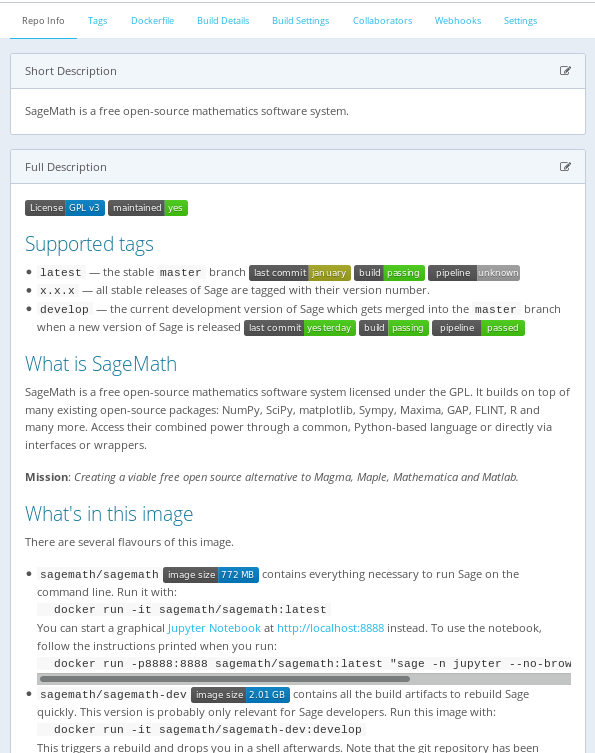
\includegraphics[width=\textwidth]{screenshots/dockerhub}
    \caption{The DockerHub landing page for Sage's Docker images, including
    up-to-date build status read from the GitLab pipeline.}
    \label{fig:sage-dockerhub}
\end{figure}


It means that recent stable \& unstable versions of Sage are automatically made
available for anybody to work with, without the need of having to understand
how to build Sage on their machine.

Sage developers can use these to reproduce and understand issues
reported by the CI system simply by downloading the container and running the
Sage version contained in that container.

Projects that depend on Sage can use these Docker containers for their own CI
needs and run their tests based on these containers. Without such Docker
containers, most such projects would refrain from using CI as setting up Sage
in a CI system appeared to be too complicated.

Sage (and projects depending on Sage) can link to these containers through
mybinder.org to make different versions of their systems available through
public web interfaces.  This means that anybody can easily experiment with the
latest unreleased features in a web browser without having to go through any
local installation.

\clearpage
\subsection{GAP}

\GAP has a mechanism for user contributions in the form of packages,
which may be submitted for refereeing and for the redistribution with \GAP.
They extend the functionality of the system and may implement mathematical
algorithms, provide mathematical databases, interfaces to other systems or
enhancements of the system's infrastructure such as tools for debugging
and profiling, and building documentation. 

Packages are developed and released independently of the core \GAP system.
They should be properly integrated into \GAP to not to break the functionality
of the system or any other package. On the other hand, changes in \GAP are only
permitted to have a disruptive effect on package functionality in a major
release, and we aim to identify such situations in advance and resolve them
in cooperation with package authors. Hence continuous integration facilities
in \GAP are designed to suit the following primary goals:
\begin{itemize}
\item checking pull requests which propose changes to the core \GAP system
\item checking for new versions of \GAP packages redistributed with \GAP;
retrieving and storing them, and combining them for testing and redistribution
\item running package integration tests which check that \GAP packages redistributed
with GAP do not break the functionality of the core \GAP system
\item wrapping and testing \GAP releases
\item testing official package releases for their readiness for the next \GAP release
\item testing package development versions for their compatibility with the \GAP development version
\end{itemize}

This is supported by the following infrastructure:
\begin{itemize}
\item Jenkins CI\footnote{Another popular framework for self-hosted CI
services; \url{https://jenkins.io/}} instance at the University of St Andrews,
providing Linux, macOS and Windows nodes (available only within St
Andrews network due to security restrictions)
\item Travis CI accounts to test builds on Linux (both on native 
Travis CI infrastructure and on Docker containers for \GAP; we
also used macOS builds in the past, but then they were disabled
due to reliability and performance issues):
\begin{itemize}
\item for the core \GAP system: \url{https://travis-ci.org/gap-system/}
\item for \GAP packages: \url{https://travis-ci.org/gap-packages/}
\end{itemize}
\item Codecov\footnote{A specialized supplement to CI systems for hosting code
 coverage reports -- that is, measures of how well a project's test suite
 tests or ``covers'' lines of code and different code branches;
 \url{https://codecov.io/}} accounts:
\begin{itemize}
\item for the core \GAP system: \url{https://codecov.io/gh/gap-system/gap}
\item for \GAP packages: \url{https://codecov.io/gh/gap-packages/}
\end{itemize}
\item AppVeyor account to test builds on Windows under Cygwin: \url{https://ci.appveyor.com/project/gap-system/gap}
\item A collection of Docker containers with various configurations available from
Docker Hub: \url{https://hub.docker.com/r/gapsystem/}
\end{itemize}
All links to critical CI builds are collected together
at \url{https://github.com/gap-system/gap-distribution}.

The core \GAP system tests use Travis CI and AppVeyor to check every pull
request submitted to the main \GAP repository on both Linux and Windows, and to
publish code coverage reports to Codecov. In the last 6 months, code coverage
on Travis CI increased from 70\% to 75\%, mainly due to new tests added by our
external collaborator Max Horn (University of Gie{\ss}en).  In addition to
that, several extended tests are performed on Jenkins, as they are more time
consuming.

\GAP package authors are advised to provide with each package a short
test suite, which may be used to check that a package works as expected,
together with metadata which informs \GAP how to run that test suite.
Such tests are run regularly as a part of the standard \GAP test suite.
Since Jenkins CI outputs are not accessible outside St Andrews, we use
a two-tier approach: new versions of \GAP packages are picked up and
tested internally on the Jenkins CI instance in St Andrews; approved
versions are then published to be used in all further tests of \GAP
(core system and package integration tests) on Travis CI, and to run
standard tests of GAP packages in a way making their output available
to their authors. These builds use Docker containers for the latest
\GAP release and for the two release branches of the \GAP repository.

For more comprehensive testing, we provide a standard Travis CI and 
Codecov setup for GAP packages, available in the \software{Example} package
\url{https://github.com/gap-packages/example}. It has been adopted and
customised by most of the \GAP packages developed on \GitHub (see their
list at \url{https://gap-packages.github.io/}). Furthermore, there are
tools for creating and publishing packages, primarily developed by our
external collaborator Max Horn:
\software{PackageMaker}\footnote{\url{https://github.com/gap-system/PackageMaker}},
\software{ReleaseTools}\footnote{\url{https://github.com/gap-system/ReleaseTools}}
and \software{GitHubPagesForGAP}\footnote{\url{https://github.com/gap-system/GitHubPagesForGAP}}.
All these measures facilitate interaction between contributors to packages
and the core GAP system, improve reliability of our software and help to
keep regular release cycles.

The following table shows the dynamics of the number of packages redistributed
with \GAP, number of authors involved in them, and adoption of standard tests
by packages included in selected \GAP releases in 2012--2018.

\begin{center}
\begin{tabular}{ |l|c|c|c| } 
\hline
GAP           & Number of    & Number     & Have standard \\
release       & of packages  & of authors & regression tests \\
\hline
4.5.4 (06/2012) &  99 & 129 & 46 \\
4.5.7 (12/2012) & 105 & 130 & 47 \\
4.6.2 (02/2013) & 106 & 133 & 58 \\
4.7.2 (12/2013) & 114 & 140 & 51 \\
4.7.6 (11/2014) & 115 & 151 & 53 \\
4.7.9 (11/2015) & 119 & 158 & 57 \\
4.8.2 (02/2016) & 131 & 167 & 69 \\
4.8.6 (11/2016) & 131 & 171 & 69 \\
4.8.9 (12/2017) & 132 & 186 & 73 \\
4.9.1 (05/2018) & 134 & 186 & 85 \\
4.9.3 (to appear) & 140 & 187 & 91 \\
\hline
\end{tabular}
\end{center} 


\subsection{Cysignals}

The Cysignals
project\footnote{\url{https://cysignals.readthedocs.io/en/latest/}} has been
using Travis CI\footnote{\url{https://travis-ci.org/sagemath/cysignals}} for
continuous integration on Linux practically since its inception (see
\longdelivref{UI}{pari-python-lib1}).  In Spring of 2018 we made
initial progress towards adding native Windows support to
Cysignals\footnote{\url{https://github.com/sagemath/cysignals/pull/76}} as well
as continuous integration for both native Windows and Cysignals on Cygwin using
AppVeyor\footnote{\url{https://github.com/sagemath/cysignals/pull/95}}, the
initial results of which have been promising.  The process of adding Cygwin
testing on AppVeyor even exposed new Cygwin-specific bugs with Cysignals that
had not been previously caught.

However, multi-platform testing still remains an interesting problem for
Cysignals in particular.  The low-level details of Cysignals are such that its
functionality can depend heavily on the underlying operating system kernel
(even different versions of the Linux kernel).  As such, one would like to be
able to test against different kernels.  Because most CI services -- including
Travis CI -- are using container-based technology, this means that even testing
different OS platforms via containers is not entirely helpful, because all
containers running on the system host system are using the same underlying
kernel. Another problem is that although Travis CI supports build
configurations using macOS, it does not support this by default for
Python-based projects without employing various unsupported workarounds.

Thus, an area for future work might be to try using GitLab's CI framework and
providing our own build runner machines (possibly even reusing the existing one
from Sage's buildbot fleet) to test Cysignals against more OS platforms with a
wider range of OS kernels than we might test otherwise.

\hypertarget{conclusion}{%
\section{Conclusion}\label{conclusion}}

There does not appear to be a one-size-fits all solution for continuous
integration.  Massive, complex projects like Sage, projects with many
third-party contributed components such as GAP, projects with low-level system
integrations like Cysignals, and everything in-between have different needs.
Between that fact, and the advancements in free-for-open-source cloud-hosted
CI providers, the idea of uniting OpenDreamKit projects under a single CI
platform (whether Buildbot as used by Sage, or something else) would not have
been practical or effective.

What does remain clear -- and is a commonality between the projects mentioned
in this report in particular, as well as others, is the need for easy access
to ``hardware'' infrastructure with which one can easily spin up a virtual
machine on which to install some operating system one does not have immediate
access to.  In the case of non-free OSes, this includes a need for easy to
obtain Windows licenses for running Windows VMs and, in the case of macOS,
specialized hardware as well, as Apple's licensing is extremely restrictive
when it comes to virtualization.  It should be noted that this need is not
strictly for the use case of continuous integration, but also for building
software releases for multiple platforms, investigation by developers of
platform-specific bugs, and new development to improve multi-platform support
in general.  For example, the author has personally experienced frustration
with obtaining access to a macOS machine in order to investigate macOS-specific
bugs in Sage, having not procured an Apple machine for personal use.

The current situation is such that individual developers must find ways to
access these kinds of computing resources, and the ease of doing so may depend
on the level of institutional resources available to them.  At Universit\'e
Paris-Sud we have found it easy to create and access VMs of free UNIX-like
operating systems, but had to put several days of FTEs into getting a Windows
VM up and running on that platform, with mixed results. And this provides us no
help for macOS.  Meanwhile the build machines for \GAP hosted at St Andrews
meet the project's needs for CI, but are not accessible outside the St Andrews
firewall and are thus not easily accessible to \GAP developers at other
institutions.  In both cases, some effort is required by the community to
maintain their build hardware infrastructure, which this work might be more
efficiently handed off to experts working in dedicated computing centers.

For example, we are discussing the possibility of getting in touch with EGI and
seeing if we might be able to use EGI-provided resources for a multi-platform
cloud environment specifically for use by open source mathematics projects.
Ideally we would want this to be provided in such a way that it isn't
restricted to projects that are strictly European by nature (or maybe at the
most have some European grant or contributors associated with it).  Or at the
very least, we would want to be able to easily create server infrastructure
for a given project which can then be shared as needed with other trusted
developers of that project.  However, the exact nature of such an arrangement
remains an open question to be resolved.

\end{document}

%%% Local Variables:
%%% mode: latex
%%% TeX-master: t
%%% End:
